\documentclass{beamer}
\usepackage[utf8]{inputenc}
\usepackage[T1]{fontenc}
\usepackage[english]{babel}
\usepackage{graphicx}
\usepackage{times}

\usetheme{AGH}

\title[]{Adaptacyjne środowisko obliczeniowe skalujące aplikacje użytkowników}

\author[D. Chrząścik, R. Morytko]{Dariusz Chrząścik\\
Radosław Morytko\\
Promotor: dr inż. Marcin Jarząb}

\date[2014]{12.06.2014}

\institute[AGH]
{Informatyka\\ 
Wydział Informatyki, Elektroniki i Telekomunikacji
}

\setbeamertemplate{itemize item}{$\maltese$}

\begin{document}

{
%\usebackgroundtemplate{
\includegraphics[width=\paperwidth]{assets/titlepage}} % wersja angielska
\usebackgroundtemplate{
\includegraphics[width=\paperwidth]{assets/titlepagepl}} % wersja polska
 \begin{frame}
   \titlepage
 \end{frame}
}


\begin{frame}
\frametitle{Plan prezentacji}

\begin{itemize}
	\item Problem
	\item Cel pracy
	\item Założenia
	\item Istniejące rozwiązania
	\item Propozycja rozwiązania
	\item Implementacja
	\item Ewaluacja
	\item Wnioski
\end{itemize}

\end{frame}



\begin{frame}
\frametitle{Problem}

\begin{itemize}
\item Minimalizacja kosztów związanych z utrzymaniem aplikacji
\item Zapewnienie odpowiedniej jakości usług dostarczanych przez aplikacje (QoS)
\item Optymalne wykorzystanie zasobów
\end{itemize}

\end{frame}




\begin{frame}
\frametitle{Cel pracy}

\begin{itemize}
\item Opracowanie sposobu na optymalne wykorzystanie zasobów

\item Stworzenie architektury referencyjnej
\item Implementacja architekutury o charakterze \textit{proof-of-concept}
\item Ewaluacja
\end{itemize}

\end{frame}





\begin{frame}
\frametitle{Założenia}

\begin{itemize}
\item Model chmury obliczeniowej
	\begin{itemize}
		\item udostępnianie środowisk wykonawczych dla aplikacji (\textit{PaaS})
		\item współpraca między chmurami
	\end{itemize}
\end{itemize}

\end{frame}





\begin{frame}
\frametitle{Istniejące rozwiązania}

\begin{itemize}
\item Carina
\item CloudFoundry

\item OneFlow
\item OpenShift
\end{itemize}

\end{frame}





\begin{frame}
\frametitle{Propozycja rozwiązania}
\framesubtitle{Adresowane problemy}

\begin{itemize}
\item Nieadekwatność akcji podejmowanych przez system
\item Zamknięcie na współprace z innymi chmurami obliczeniowymi
\item Pasywne podejście do problemu skalowania aplikacji 
\end{itemize}

\end{frame}



\begin{frame}
\frametitle{Propozycja rozwiązania}
\framesubtitle{Adresowane problemy}

\begin{itemize}
\item Nieadekwatność akcji podejmowanych przez system
		\begin{itemize}
			\item dopasowanie akcji do zaobserwowanego problemu
		\end{itemize}

\item Zamknięcie na współprace z innymi chmurami obliczeniowymi
		\begin{itemize}
			\item kooperacja z innymi chmurami obliczeniowymi
		\end{itemize}

\item Pasywne podejście do problemu skalowania aplikacji 
		\begin{itemize}
			\item analiza skutków podejmowanych wcześniej akcji
		\end{itemize}		
\end{itemize}
\end{frame}




\begin{frame}
\frametitle{Propozycja rozwiązania}

\begin{itemize}
	\item System adaptacyjny adresujący wspomniane problemy
	\item System zbudowany w oparciu o model autonomicznego systemu autorstwa IBM
\end{itemize}


\end{frame}





\begin{frame}
\frametitle{Propozycja rozwiązania}
\framesubtitle{Kontekst użycia systemu}
\vspace{2 mm}
\begin{center}

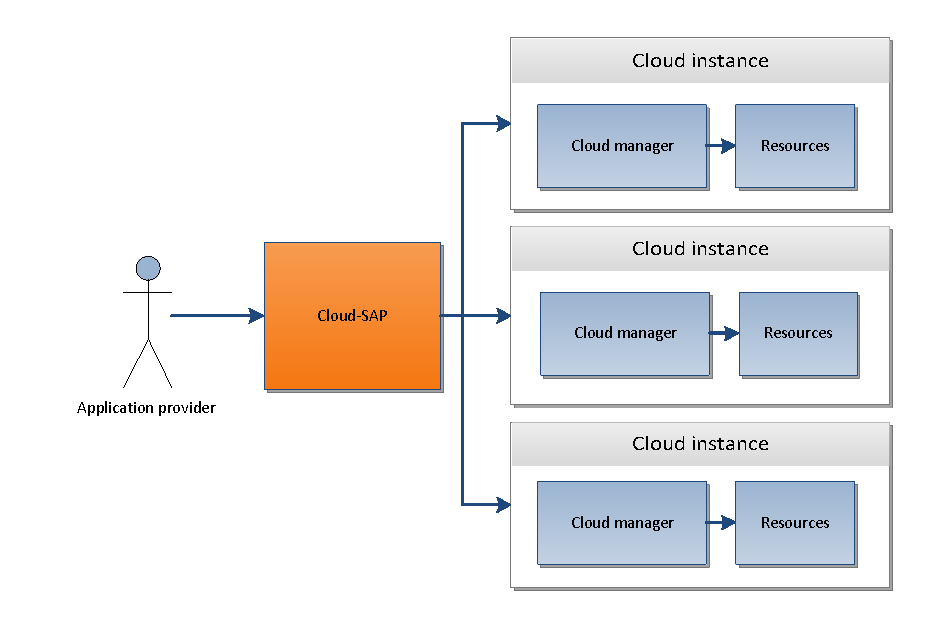
\includegraphics[width=0.8\textwidth]{assets/csap-usage-context}
\end{center}

\end{frame}



\begin{frame}
\frametitle{Propozycja rozwiązania}
\framesubtitle{Model warstwowy systemu}
\vspace{2 mm}
\begin{center}
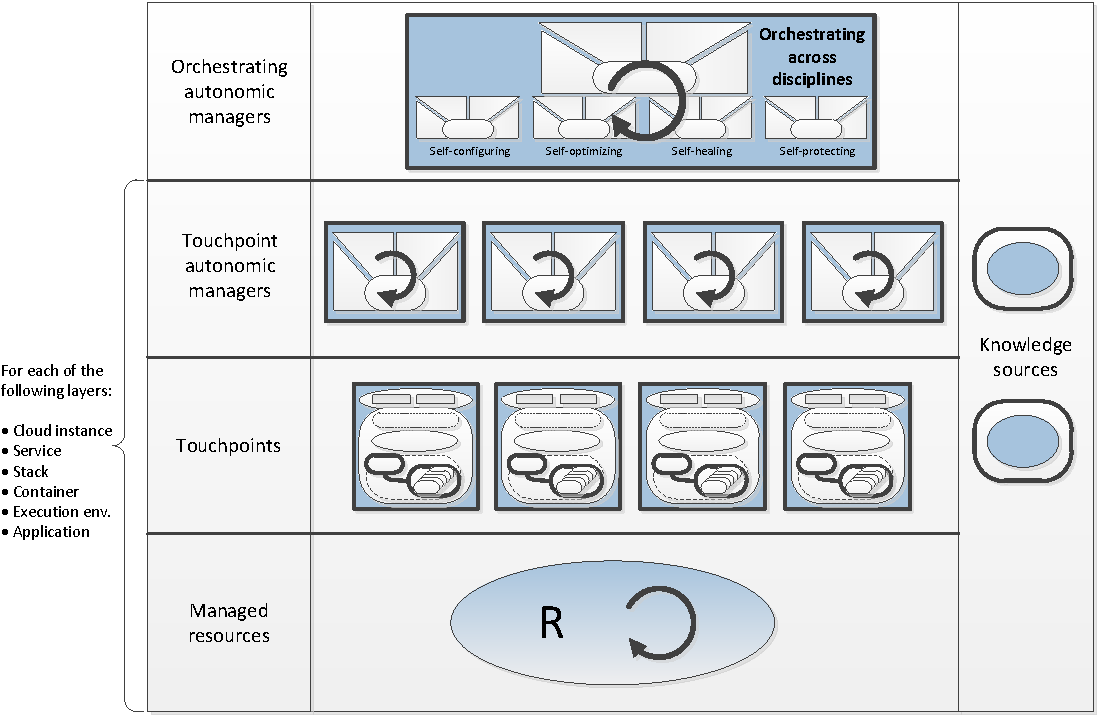
\includegraphics[width=0.8\textwidth]{assets/csap-layers}
\end{center}
\end{frame}



\begin{frame}
\frametitle{Implementacja}

\vspace{2 mm}
\begin{center}
\includegraphics[width=0.9\textwidth]{assets/hlo-implementation}
\end{center}
\end{frame}



\begin{frame}
\frametitle{Ewaluacja}
\framesubtitle{Środowisko testowe}

\end{frame}




\begin{frame}
\frametitle{Ewaluacja}
\framesubtitle{Automatyczne skalowanie}

\begin{center}
\includegraphics[width=0.9\textwidth]{assets/auto-scaling-1cp-cost-comparison}
\end{center}


\end{frame}



\begin{frame}
\frametitle{Ewaluacja}
\framesubtitle{Automatyczne skalowanie: wielu dostawców}

\begin{center}
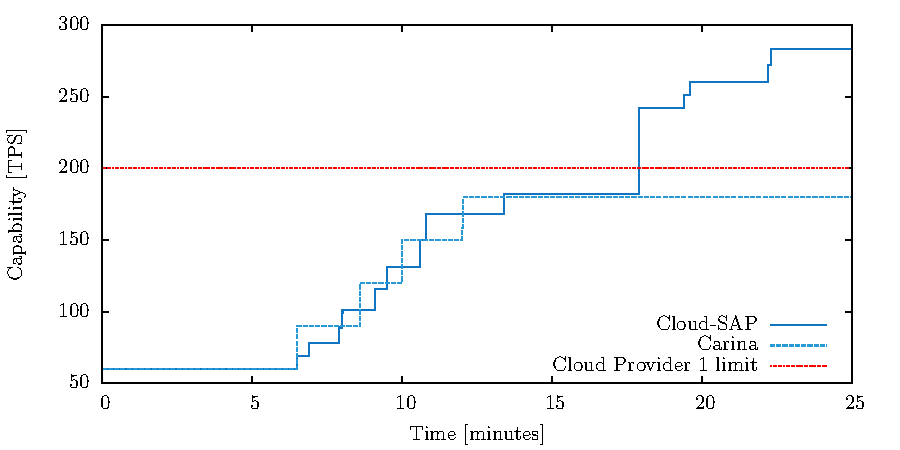
\includegraphics[width=0.9\textwidth]{assets/auto-scaling-2cp-tps-comparison}
\end{center}

\end{frame}


\begin{frame}
\frametitle{Ewaluacja}
\framesubtitle{Pozostałe przypadki testowe}

\begin{itemize}
	\item Koszt tworzenia środowiska wykonawczego aplikacji
	\item Czas tworzenia środowiska wykonawczego aplikacji
\end{itemize}

\end{frame}


\begin{frame}
\frametitle{Wnioski}

\begin{itemize}
	\item Cele zostały osiągnięte
	\item Dalsze prace
		\begin{itemize}
			\item rozszerzenie implementacji o bardziej zaawansowane mechanizmy
			\item zainteresowanie społeczności open-source 
		\end{itemize}
\end{itemize}

\end{frame}






\end{document}

